Below are the results of the low pass filter. The measured frequencies and amplitudes are then plotted on a bode plot.

\begin{adjustwidth}{-2.5 cm}{-2.5 cm}\centering\begin{threeparttable}[!htb]
        \scriptsize
        \begin{tabular}{lrrrrr}\toprule
            \textbf{Input Amplitude(in V)} & \textbf{Output Amplitude(in V)} & \textbf{Phase(in deg)} & \textbf{Frequency(in Hz)} & \textbf{Amplitude(in dB)} \\\midrule
            10.1                           & 10                              & -0.36                  & 50                        & 20.00                     \\
            10.1                           & 10                              & -0.36                  & 100                       & 20.00                     \\
            10.1                           & 10                              & -2.59                  & 200                       & 20.00                     \\
            10.2                           & 10                              & -6.49                  & 500                       & 20.00                     \\
            10.4                           & 10.1                            & -11.8                  & 1000                      & 20.09                     \\
            10.9                           & 10                              & -23                    & 2000                      & 20.00                     \\
            12.2                           & 8                               & -47.4                  & 5000                      & 18.06                     \\
            11.8                           & 5.04                            & -64                    & 10000                     & 14.05                     \\
            12.4                           & 2.8                             & -75.3                  & 20000                     & 8.94                      \\
            11.8                           & 1.14                            & -82.8                  & 50000                     & 1.14                      \\
            11.8                           & 0.596                           & -84.6                  & 100000                    & -4.50                     \\
            \bottomrule
        \end{tabular}
        \caption{The measured frequencies and amplitudes from the low pass filter.}\label{tab: }
    \end{threeparttable}\end{adjustwidth}


\begin{figure}[H]
    \centering
    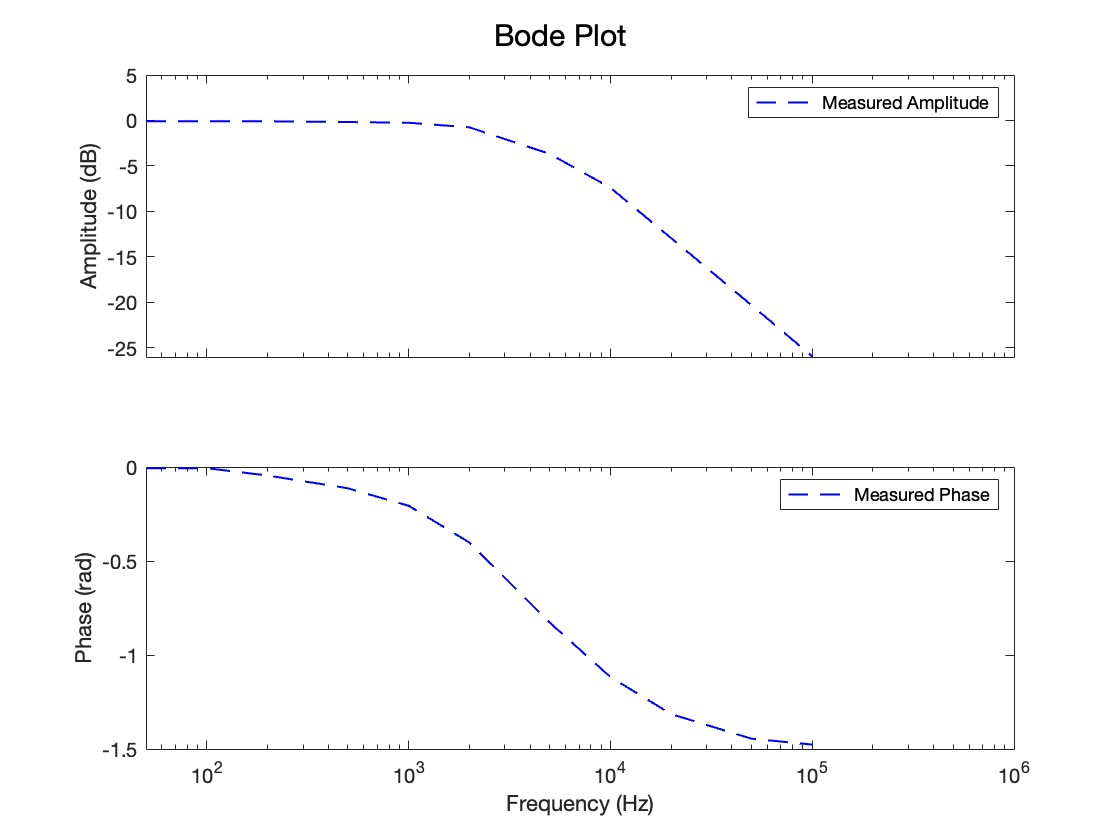
\includegraphics[scale=0.30]{images/bode_plot_low_pass_measured.jpg}
    \caption{Bode plot of measured frequencies, amplitudes and phase shifts of the low pass filter.}
\end{figure}

The calculated cutoff frequency can be obtained by the following relation for the low pass filter circuit:
\begin{equation}
    f_{-3dB} = \frac{1}{2\pi RC}
\end{equation}